\clearpage

\section*{\scalefont{1.2}Appendix}


\section{Quality and efficiency of BLOOM with 8-bit quantization}\label{appendix:8bit_quality}

\begin{table}[b]
\begin{minipage}{0.56\textwidth}
\centering
\caption{Zero-shot accuracy for \mbox{BLOOM-176B} and \mbox{OPT-175B} with 8-bit and 16-bit weights.\nocite{eval-harness}}
\vspace{9pt}
\resizebox{\linewidth}{!}{%
\begin{tabular}{lccccc}\toprule
\textbf{Model}            & \textbf{Bits} & \textbf{HellaSwag} & \textbf{LAMBADA} & \textbf{WinoGrande} & \textbf{Avg}             \\\midrule
\multirow{2}{*}{BLOOM}    & 16            & 73.0               & 67.2             & 70.1                & 70.1                     \\
                          & 8             & 72.8               & 68.1             & 70.1                & 70.3                    \\\midrule
\multirow{2}{*}{OPT} & 16            & 78.5               & 74.7             & 72.6                & 75.3                     \\
                          & 8             & 78.5               & 74.6             & 71.7                & \multicolumn{1}{r}{74.9} \\\bottomrule
\end{tabular}
}
\label{tab:quality}
\end{minipage}
\hspace{4px}
\begin{minipage}{0.42\textwidth}
\centering
\caption{Generation throughput (tokens/s) for BLOOM-176B with 8-bit and 16-bit weights on 8$\times$~A100 GPUs.}
\label{tbl:memory_footprint}
\resizebox{0.75\linewidth}{!}{%
\begin{tabular}{lccc}\toprule
\multirow{2}{*}{\bf Weights}& \multicolumn{3}{c}{\bf Batch size} \\\cmidrule{2-4} & \bf 1 & \bf 8 &\bf 32  \\\toprule
16-bit       & 4.18 & 31.3  & 100.6  \\
8-bit        & 3.95 & 29.4  & 95.8\\\bottomrule
\end{tabular}
}
\label{tab:throughput}
\end{minipage}
\end{table}

As shown in Table~\ref{tab:quality}, this method has little effect on LLM quality for major benchmarks.
In terms of inference time, Table~\ref{tab:throughput} demonstrates that quantization has about $5\%$ of overhead with batch size 1 (20 tokens), but becomes negligible for larger batches.




\section{Estimating theoretical best throughput with RAM offloading}\label{appendix:offloading_estimate}
In this estimate, we use the best possible hardware setup for offloading: CPU RAM offloading via PCIe 4.0 with 16 PCIe lanes per GPU.
In 8-bit, the model uses 1 GB of memory per billion parameters, and PCIe~4.0 with 16 lanes has a throughput of 256 Gbit/s. We assume an offloading latency of zero in the upper bound estimation. As such, offloading 176B parameters takes at least:
$$\frac{176 \text{ GB} \cdot 8}{256 \text{ Gbit/s}} = 5.5\text{ seconds}$$
This gives the upper bound of $1 / 5.5 \approx 0.18$ tokens/s for the inference speed.

\section{Extension to beam search algorithms}\label{appendix:beam_search}

There are several variations of beam-search algorithm used for language model inference, including standard beam search, diverse beam search, constrained beam search, and more. A common thread between those algorithms is that they maintain a fixed number $k$ of candidate sequences between steps. These sequences are informally referred to as the ``beam''. On every step, these algorithms generate possible continuations of sequences in the previous beam, then use some fitness criterion to select $k$ of these continuations for the next beam.

From a computational point of view, this procedure is similar to simple ``greedy'' inference with a batch of $k$ sequences. However, there is one important difference: unlike batched inference, beam search algorithms can ``shuffle'' candidate sequences between steps. In other words, 3rd best sequence from time step $t$ can produce 1st or 2nd (or any other) sequence on the next step. Furthermore, a single sequence on time step $t$ can produce multiple sequences selected for step $t+1$.

Since different beam search variantions use different criteria for selecting top sequences, we need a generic algorithm that can fit any criterion. In our system, we implement this by allowing clients to reorder server-side attention cache after each step. Formally, a client can send a list of at most $k$ integers in range $[1, k]$, where i-th index specifies which previous attention cache should be used when generating $i$-th sequence of the next beam.

For instance, when given indices $[2, 2, 1, 3, 2]$, a server will use 2nd best sequence from step $t$ to produce the new 1st, 3rd and 5th best sequences. Previous 1st and 3rd best sequences go to 3rd and 4th places, respectively. Finally, previous 4th and 5th sequences are discarded. From a technical point of view, servers implement this reordering by reordering attention cache with the specified indices (\texttt{torch.gather} operation) immediately before performing an inference step.



\section{Details of the server load balancing algorithms}\label{appendix:load_balancing_algo}

\paragraph{Measuring throughput.} Before joining for the first time, each server measures its Internet connection throughput (in tokens/second, using one of public web APIs for doing that) and GPU throughput (in tokens/second, using a small benchmark running several forward passes). The minimum of these values becomes the overall server throughput, which is then cached for future runs.

\paragraph{Initial block assignment.} We assume that each server holds a segment of \textbf{consecutive} transformer blocks to minimize inference latency. Clients may request to perform a forward or backward pass for the whole segment of blocks or its subsegment, if necessary. Normally, each server loads as many blocks as it can fit in its GPU memory, unless a user limits the number of blocks to utilize the rest of memory for something else.

Before starting, each server calculates the values of $t_i$~-- the total throughput of servers currently holding the $i$-th block or loading it (to start holding it in a few minutes). Then, to find the best segment of blocks to serve, the server looks for the most narrow bottleneck in the network. Formally, if the model has $L$ blocks and the server can hold $K$ of them in its GPU memory, we calculate:
\begin{equation}\label{eqn:load_balancing}
start=\underset{i=1}{\overset{L-K+1}{\arg\min}} \quad \mathrm{sorted}([t_i,\ t_{i+1},\ \ldots,\ t_{i+K-1}])
\end{equation}
Here, $\arg\min$ compares the sorted arrays lexicographically and chooses the leftmost $start$ in case of multiple minimums.

This way, the next joining server would always cover a block with the smallest $t_i$. If there are multiple bottlenecks like this, the server will try to cover as many of them as possible (we choose to cover the minimums first because the overall throughput is the minimum of throughputs among model blocks). Among the remaining options, we choose a segment covering as many second minimums as possible, and so on.

\paragraph{Quality of block assignment.} While we are not aware of the exact polynomial-time solution for the problem of assigning the segments optimally, we have conducted computational experiments and found out that this greedy algorithm (running in polynomial time) usually finds an assignment with total throughput of 90-100\% of the optimal one (found by trying out all possible assignments in exponential time), given that the values of throughput are realistic to our setup.

\paragraph{Rebalancing.} Since servers may leave at any time, each server also periodically checks if the current assignment is "good enough" compared to the throughput estimated by running the greedy solution for servers currently present in the network.

Formally, each server periodically looks for a segment of blocks that is more appropriate than the currently loaded blocks with respect to the $\arg\min$ rule~(\ref{eqn:load_balancing}). If it finds one, it simulates how the rest of the servers would behave if we replace the current blocks with the new ones (how other servers would change their blocks afterwards). If the eventual throughput is at least $p\%$ better, the server commits to the change and announces that it changes the blocks, then other servers do the rest of the changes (eventually increasing the total throughput).

We use $p=20\%$ since it gives a reasonable trade-off between the swarm throughput and the frequency of block replacements in our experiments (see Appendix~\ref{appendix:load_balancing_exps}). Specifically, a lower value of $p$ leads to block replacements happening too often, which negatively affects the inference latency since each block replacement resets attention caches for this block.

\paragraph{Stability of the greedy algorithm.} The rebalancing algorithm does not cause oscillations since a series of block replacements is executed only if it leads to eventually increasing throughput by at least $p\%$. Once a "good enough" throughput is achieved, servers do not change their blocks anymore (unless an essential number of servers join or leave). We verified this behavior computationally, simulating a network with thousands of servers with different throughputs.

To conclude, this greedy heuristic allows servers to quickly close the gaps if a substantial share (up to 100\%) of servers holding certain blocks leave, but avoids excess block replacements otherwise.

\begin{figure*}[tb]
    \centering
    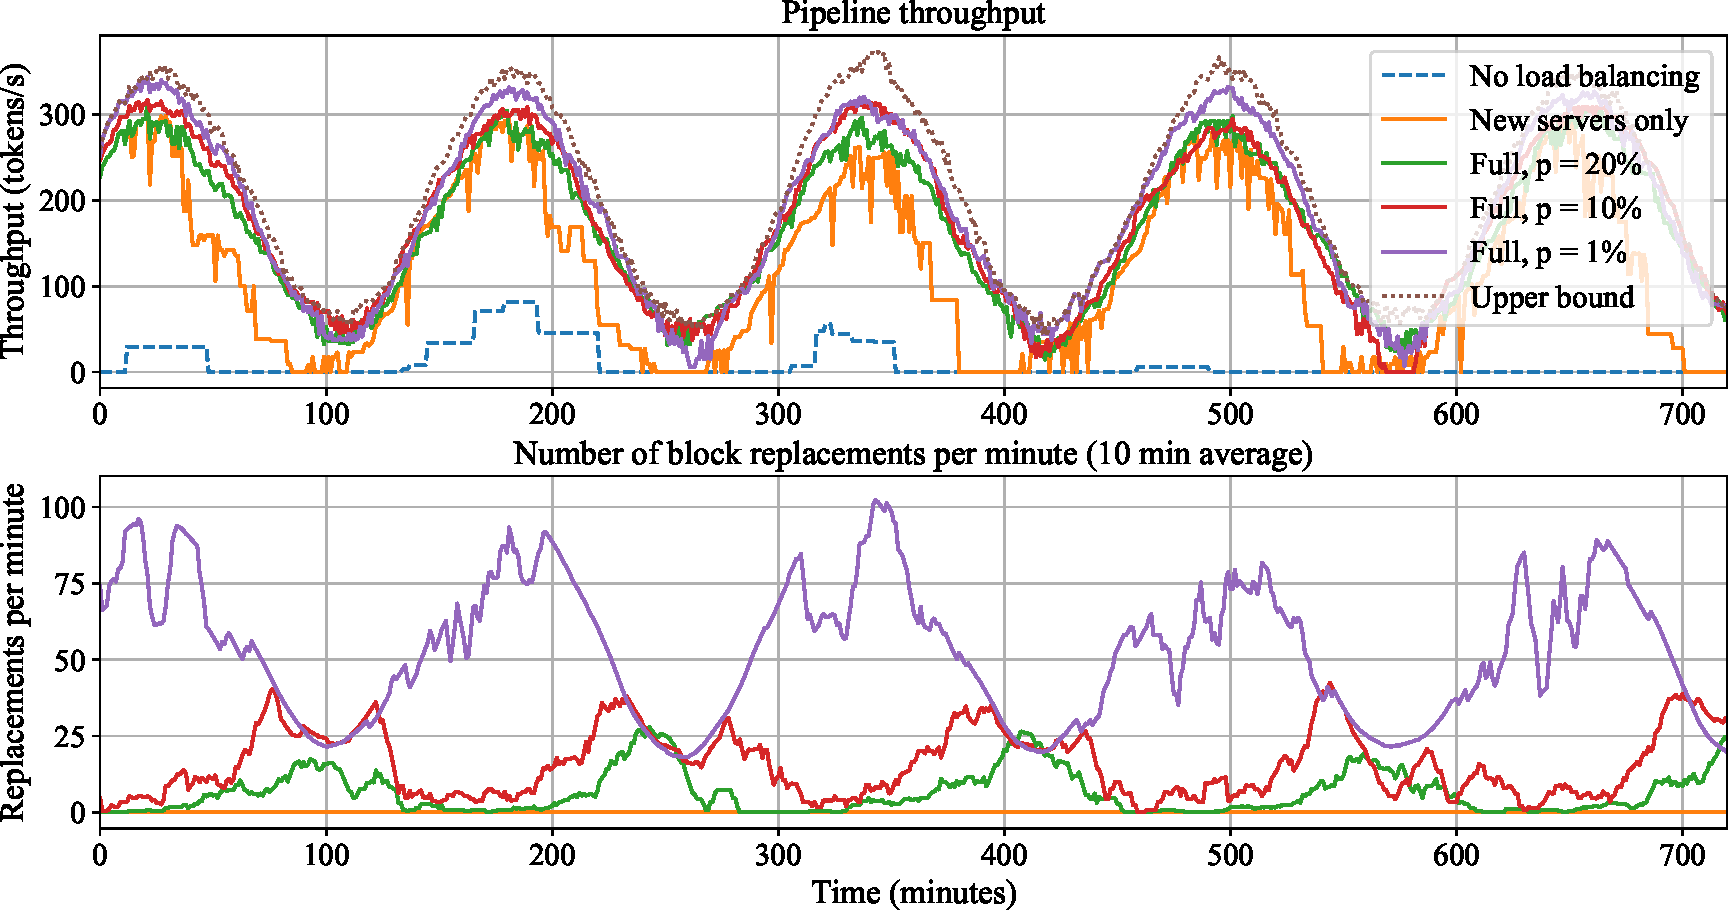
\includegraphics[width=\linewidth]{resources/load_balancing_exps.pdf}
    \vspace{-12pt}
    \caption{Behavior of the load balancing algorithms evaluated in Appendix~\ref{appendix:load_balancing_exps}.}
    \label{fig:load_balancing_exps}
    \vspace{-6px}
\end{figure*}


\section{Evaluation of the server load balancing algorithms}\label{appendix:load_balancing_exps}

In this section, we measure the effectiveness of the load balancing algorithm used in our system. We run all experiments using a fleet of 206 virtual instances that simulate participants. To keep experiment costs manageable, we do not use GPUs for this evaluation, instead simulating uneven server throughput programmatically. For each server, we sample its throughput from the uniform distribution $t \sim \mathbb{U}[0, 100]$ tokens/second, then sample its memory size so it can hold $b \sim \mathbb{U}[1, 10]$ blocks (out of 70 blocks in total, as in BLOOM-176B).

Each server follows a certain availability schedule, i.e. turns on and shuts down at the same predefined time across all experiments.
We assign these schedules such that the number of active servers follows a sine wave, simulating daily activity cycles.
The schedule has approximately 100--110 active servers during peak activity and 15--25 servers at its lowest points.
Note that each peak contains a different subset of 100--110 active servers out of 206 instances in total.

We evaluate the following approaches to load balancing:
\begin{enumerate}
  \vspace{-1px}
  \item \textbf{No load balancing} -- a baseline system where servers load a random contiguous interval of model blocks.
  \vspace{-1px}
  \item \textbf{Balancing new servers only} -- a simplified load balancing where servers choose the optimal blocks when joining the swarm (using the rule~(\ref{eqn:load_balancing}) from Appendix~\ref{appendix:load_balancing_algo}) but never change them.
  \vspace{-1px}
  \item \textbf{Full load balancing} -- the full algorithm, where every minute each server checks if they need to replace their blocks. We use the efficiency threshold $p$ (as described in Appendix~\ref{appendix:load_balancing_algo}) to avoid excess block replacements.
  \vspace{-1px}
  \item \textbf{Upper bound} --- the best-case throughput estimate that reassigns contiguous block segments to servers optimally every minute.
  \vspace{-1px}
\end{enumerate}

We report their behavior in Figure~\ref{fig:load_balancing_exps}. The full load balancing maintains connectivity throughout the experiment and achieves throughput close to the upper bound (staying within the 10--15\% range most of the time). Higher thresholds $p$ perform slightly worse during peak times but require only relatively infrequent block replacements, unlike the case with $p=1\%$. Note that using the assignment leading to the upper bound is not possible in practice since it requires each server to load a different set of layers every minute, on top of solving the computationally expensive optimization problem.

Curiously, the baseline running load balancing for \textit{new servers only} achieves reasonable throughput during periods where servers are actively joining. However, it quickly loses throughput when random servers leave, since this creates ``bottlenecks'' in the pipeline that require rebalancing of existing peers. Finally, the naive baseline with random layer assignment has zero throughput most of the time because it is unable to form a complete pipeline.

\section{Experiments with a wider range of failure rates}\label{appendix:failure_rate_plots}

In this section, we follow the setup from Section~\ref{sect:experiments_basic} and provide additional evaluations for a wider range of failure rates (up to 5\%) and sequence lengths (up to 2048 tokens). The results are shown in Figure~\ref{fig:failure_rate_plots}. Unlike baselines, our algorithm provides reasonable performance \textit{in all tested conditions}, especially for higher failure rates common for communicating over the Internet, using spot/preemptible instances or unreliable hardware).

\begin{figure}[H]
    \centering
    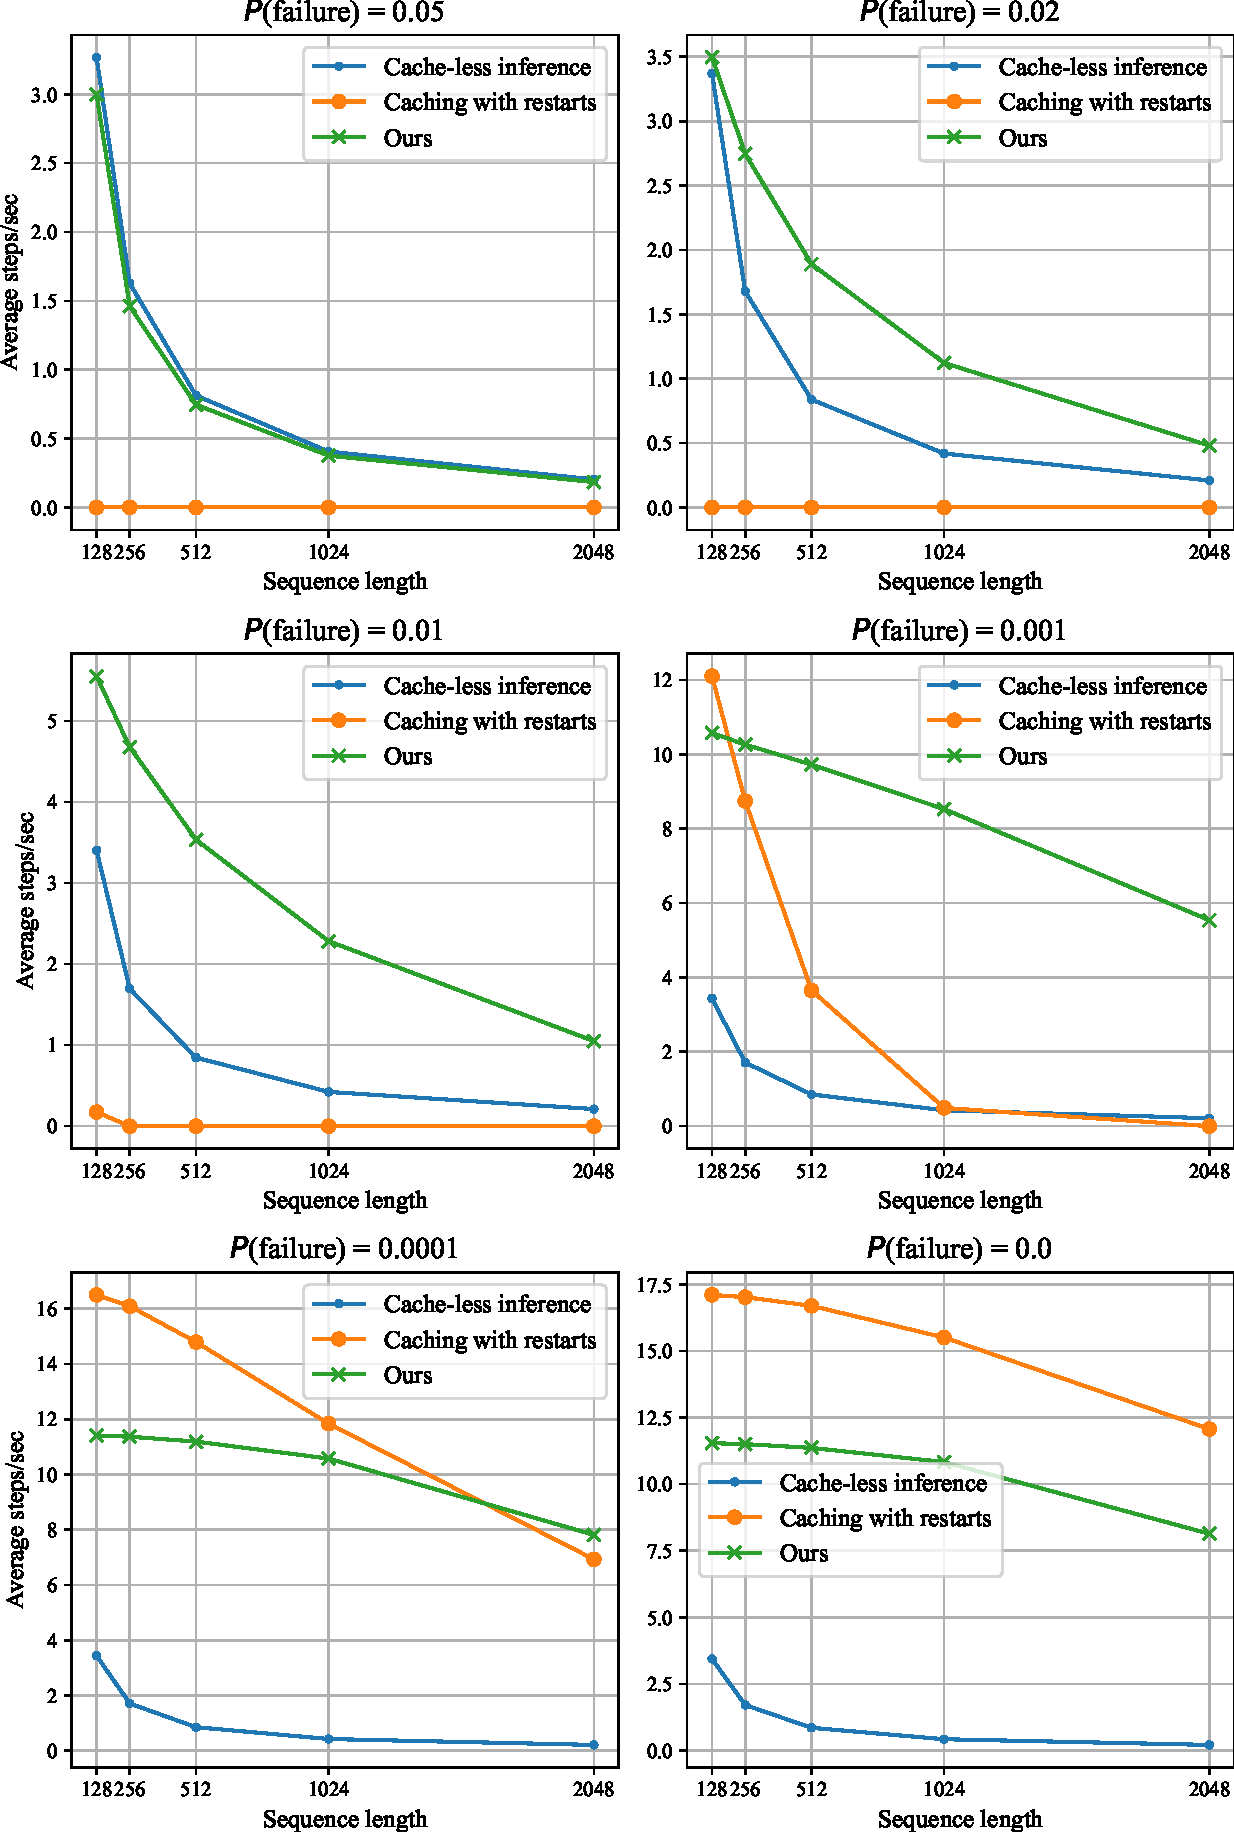
\includegraphics[width=0.875 \linewidth]{resources/pretty_failure_rate_plots.pdf}
    \caption{Sequential inference speed (steps/s) for BLOOM (7.1B) with varying failure rates. The setup is the same as in Section~\ref{sect:experiments_basic}. A failure rate $p$ means that sending a set of activations to the next pipeline stage fails with probability $p$. Zero speed means that the baseline did not finish within 1 hour.}
    \label{fig:failure_rate_plots}
\end{figure}

\section{Performance of training-time forward and backward passes}\label{appendix:backward_pass}

In this section, we evaluate throughput of training-time forward and backward passes and study factors that affect their performance. We will only consider BLOOM-176B and the ``3$\times$ A100, 1~Gbit/s'' setup from Section~\ref{sect:experiments_controlled} and focus on finetuning-specific hyperparameters, since the influence of network bandwidth and latency has already been discussed in the main paper.

\paragraph{Sequence classification.} First, we consider fine-tuning the model on a binary classification task. We take BLOOM-176B, replace the logit layer with a trainable classification head (similar to \texttt{transformers.BloomForSequenceClassification}), and add trainable prompts before the input sequence, then train the model on batches of 128-token sequences. We try \textbf{(a)} both prompt tuning and prefix tuning (involving ``deep'' prompts), \textbf{(b)} two batch sizes (8 and 32), and \textbf{(c)} two prompt lengths (16 and 4). The client shares 8 CPU cores with one of the servers and does not use the GPU.

The results are provided in Table~\ref{tbl:exp_full_step}. The prefix tuning turns out to be slower, since it adds several times more trainable parameters. Increasing prompt length and decreasing batch size also make training slower. Notably, we observe that moving client-side computations to GPU does not visibly improve performance, since the client does not perform any heavy operations in this setup\footnote{In case of sequence classification, the heaviest operation the client does is multiplying $2 \times h$ and $h \times b$ matrices, where $h$ is the hidden dimension (14336 in BLOOM-176B) and $b$ is the batch size.}.

\paragraph{Language modeling.} Next, we consider fine-tuning the model on a causal language modeling task. We take BLOOM-176B, keep the logit layer, and add trainable prompts before the input sequence. We explore the same hyperparameters as with sequence classification.

We observe that the throughput of the GPU-enabled client is similar (within 10\% difference) to the throughput in case of sequence classification, reported in Table~\ref{tbl:exp_full_step}. Indeed, the client performs only a small share of GPU computations in the forward and backward passes, and a particular model head and a loss function do not have decisive influence on the performance. However, performance of the CPU-only client turns out to be 5-10 times worse in this setup, since the client has to multiply the output embedding matrix to the hidden states of all tokens in the batch. This operation is too large to be efficiently computed on CPU\footnote{In case of language modeling, the client has to multiply $d \times h$ and $h \times b$ matrices, where $d$ is the token vocabulary size (250880 in BLOOM-176B). This is $\approx 10^5$ times more FLOPS than used in case of sequence classification.}.

\begin{table}[tb]
  \centering
 \caption{Throughput (tokens/sec) of forward and backward passes for different tasks, batch sizes, prefix lengths.}
 \label{tbl:exp_full_step}
\setlength{\tabcolsep}{3pt}
\begin{tabular}{ccccc}\toprule
\multirow{2}{*}{\bf{Mode}} & \multirow{2}{*}{\bf{Batch size}} & \multirow{2}{*}{\bf{Prompt length}} & \bf{Forward pass} & \bf{Backward pass} \\
& & & \bf{throughput}  & \bf{throughput} \\
\midrule
\multirow{4}{*}{Prompt tuning}
& 8 & 16 & 195.6 & 57.4 \\
& 8 & 4 & 213.2 & 60.8 \\
& 32 & 16 & 272.6 & 82.8 \\
& 32 & 4 & 293.1 & 84.7 \\
\midrule
& 8 & 16 & 111.0 & 42.0 \\
Prefix tuning & 8 & 4 & 178.7 & 57.8 \\
(i.e., ``deep'' prompt tuning) & 32 & 16 & 164.1 & 64.4 \\
& 32 & 4 & 255.8 & 84.8 \\
\bottomrule
\end{tabular}
\end{table}











\section*{Broader Impact}
\label{sect:broader}
\vspace{-4px}

The approach proposed in this work is only a prototype with limited direct consequences, but the long-term goal of training huge models with volunteer computing can have a lasting effect on both the research community and the general public.

\vspace{-6px}
\subsection*{Funding bias vs crowdsourcing bias} 
\vspace{-6px}
The main positive outcome we pursue is to let researchers harness volunteer computing and train models on the scale currently available only to large corporations. Ideally, a deep learning researcher with a promising idea will be able to amass the computation needed to realize this idea by involving volunteers. However, the project's appeal for volunteers depends on many factors such as subject area, current societal trends, and even researcher's personality.

For example, a project about teaching agents to play games~\cite{lc0} or fighting global pandemics~\cite{folding_covid} is likely to attract more resources than deep learning applied to soil science. In essence, volunteer computing is biased towards exciting or socially relevant research the same way as traditional HPC is biased towards the interests of those who fund it.

\vspace{-6px}
\subsection*{Alternative use and misuse} 
\vspace{-6px}
The proposed technology can be used with different economic models. If a deep learning system is immediately useful (e.g. for machine translation, information retrieval, etc), the participants could use it for their needs based on their contributions to training. This can take many forms: several labs combining their hardware and training larger models; a web-service that lets people contribute their compute instead of using ads/subscriptions; or simply a framework that someone can use to run distributed training across two or more datacenters.

Unfortunately, this also allows several opportunities for malicious use. If a machine is hacked, the attacker can use its compute unnoticed by the machine owner --- much the same way that botnets are currently used to mine cryptocurrencies. Furthermore, due to decentalized nature even legitimate Learning@home projects can be hijacked by hackers.

\vspace{-6px}
\subsection*{Security} 
\vspace{-6px}
Using crowdsourced hardware makes Learning@home susceptible to attacks from malicious participants. There are multiple attack vectors already known in P2P community: denial of service attacks, Sybil attacks, Eclipse attacks and more \cite{urdaneta2011survey, sybil_attacks_dht, dos_resistance, sybil_nodes}. Fortunately, there are variations of the DHT protocol that make it resistant to said attacks: if a reader wishes to learn more about DHT security, we recommend starting with \cite{urdaneta2011survey}.

Another source of vulnerability stems from the sequential nature of neural networks. If a single expert were to return incorrect (e.g. NaN) outputs or gradients, it could compromise the outputs of the entire network and even poison adjacent nodes through backpropagation. Recent studies expose similar attack patterns on federated learning systems \cite{bagdasaryan2018backdoor, bhagoji2018analyzing}.

The redundant nature of mixture-of-experts layers provides some degree of resistance against those attacks. A single malicious expert will only affect a small fraction of inputs that pass through this specific expert. Furthermore, a trainer with access to predictions from multiple experts could provide a higher degree of robustness by using statistical techniques (e.g., by ignoring outlier gradients). However, such techniques need to be carefully designed so as not to introduce harmful side effects.

\vspace{-6px}
\subsection*{The burden on the network} 
\vspace{-6px}
Finally, we would like to point out the potential harm that our approach can do to network infrastructure. The experiments we ran in Section \ref{sect:exp_throughput} saturate with the bandwidth of $100-200$Mbps, most of which is tensors passed between experts and trainers. 

This coincides with the typical home internet speed available in major cities of developed countries. However, not all ISPs design their infrastructure for users who always use up all their bandwidth. If too many Learning@home participants are located in one LAN or MAN, it can cause congestion or even failures in the network infrastructure. 

Similar situations frequently took place in late 2000s due to growing popularity of BitTorrent for file sharing. Fortunately, the network infrastructure is continually improving, which leads us to believe that this problem will eventually be solved. Until then, we describe several ways to reduce network load of Learning@home in Appendix E.


